\documentclass[tikz,border=10pt]{standalone}
\usepackage{helvet}
\renewcommand{\familydefault}{\sfdefault}
\usepackage{tikz}
\usepackage{amsmath}
\usetikzlibrary{positioning, arrows.meta, calc, shapes.geometric, fit, backgrounds, decorations.pathreplacing}

% Define colors
\definecolor{emeraldpine}{HTML}{1A4D3E}
\definecolor{harvardcrimson}{HTML}{A51C30}
\definecolor{ethdarkblue}{HTML}{1F407A}
\definecolor{ethpetrol}{HTML}{007A87}
\definecolor{ethbronze}{HTML}{B87333}
\definecolor{ethpurple}{HTML}{5B4B8A}
\definecolor{ink}{HTML}{1A202C}
\definecolor{softink}{HTML}{4A5568}
\definecolor{paleink}{HTML}{A0AEC0}
\definecolor{cardbg}{HTML}{F8FAFC}
\definecolor{shadecolor}{HTML}{F4F6F9}

% Rung colors from SVG
\definecolor{r1bg}{HTML}{F0FDF4}
\definecolor{r1border}{HTML}{86EFAC}
\definecolor{r1text}{HTML}{065F46}

\definecolor{r2bg}{HTML}{F8FAFC}
\definecolor{r2border}{HTML}{CBD5E1}

\definecolor{r3bg}{HTML}{FFFBEB}
\definecolor{r3border}{HTML}{FDE68A}
\definecolor{r3text}{HTML}{92400E}

\definecolor{r4bg}{HTML}{FEF2F2}
\definecolor{r4border}{HTML}{FCA5A5}
\definecolor{r4alert}{HTML}{FEE2E2}

\begin{document}
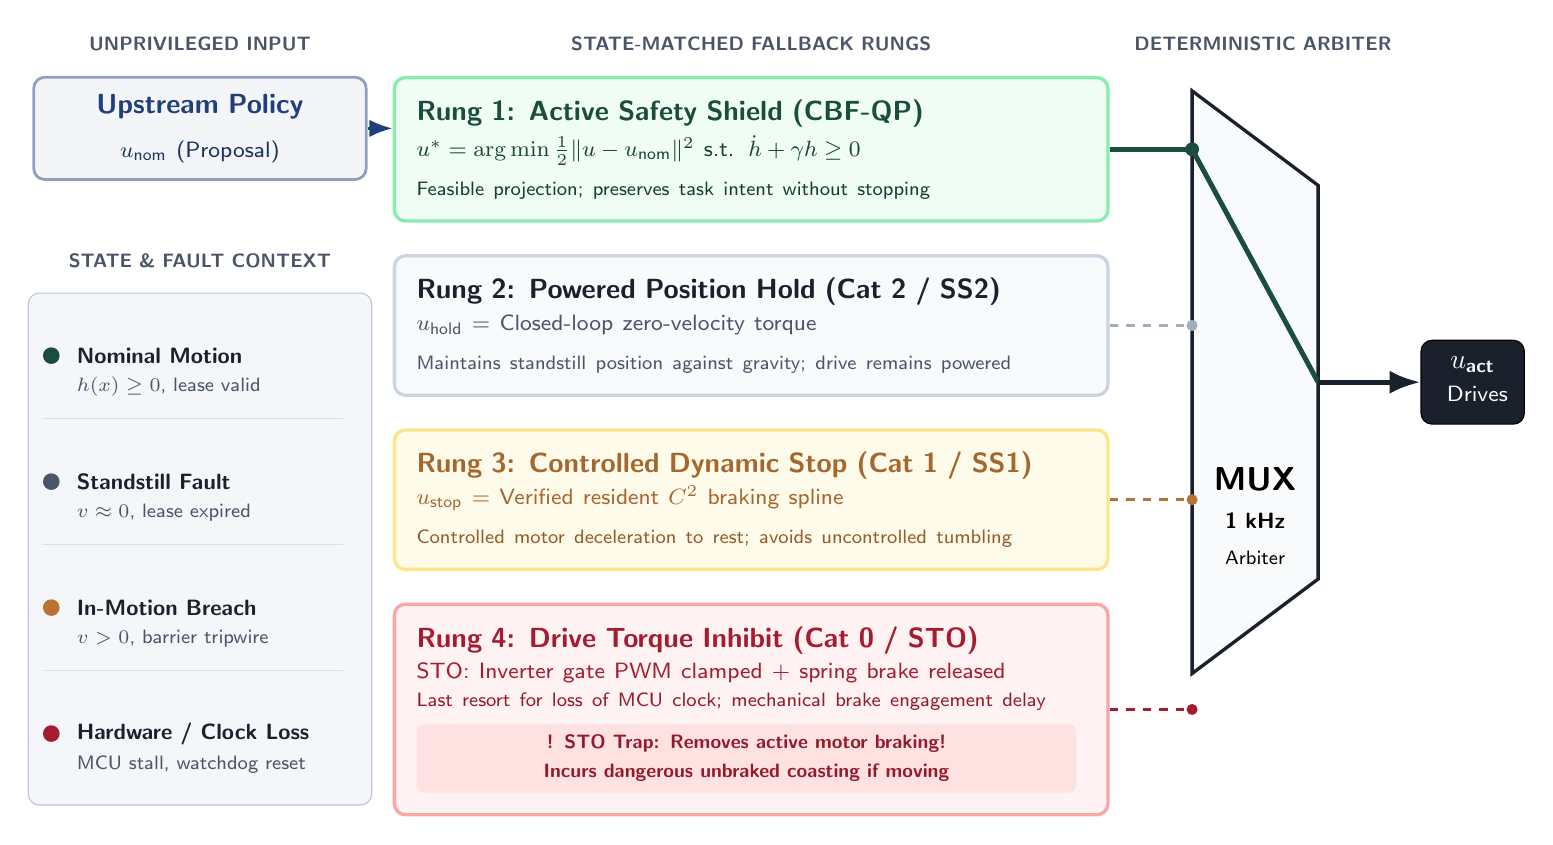
\begin{tikzpicture}[
    >=Latex,
    font=\sffamily,
    box/.style={
        draw, rounded corners=4pt, fill=cardbg, text=ink,
        align=center, inner sep=6pt
    },
    rung/.style={
        draw, rounded corners=4pt, align=left, inner sep=8pt,
        text width=8.5cm
    },
    contextbox/.style={
        draw=paleink!70, rounded corners=4pt, fill=shadecolor,
        inner sep=8pt, align=left,
        text width=3.8cm
    },
    hdr/.style={
        font=\scriptsize\bfseries, text=softink
    }
]

% ==================
% LEFT COLUMN
% ==================
\node[hdr] (hdr_input) at (0, 0) {UNPRIVILEGED INPUT};

\node[box, draw=ethdarkblue!50, fill=ethdarkblue!5, text width=3.8cm, below=0.2cm of hdr_input, line width=1pt] (input) {
    \textbf{\color{ethdarkblue} Upstream Policy}\\
    \vspace{4pt}
    \footnotesize \color{ethdarkblue!80!black} $u_{\text{nom}}$ (Proposal)
};

\node[hdr, below=0.8cm of input] (hdr_context) {STATE \& FAULT CONTEXT};

\node[contextbox, below=0.2cm of hdr_context, minimum height=6.5cm] (context) {};

% Triggers inside context box
\coordinate (c_start) at ([yshift=-0.8cm, xshift=0.3cm]context.north west);

% Trigger 1
\fill[emeraldpine] (c_start) circle (3pt);
\node[anchor=west, text=ink, font=\footnotesize\bfseries] at ([xshift=0.2cm]c_start) {Nominal Motion};
\node[anchor=west, text=softink, font=\scriptsize] (t1_desc) at ([xshift=0.2cm, yshift=-0.4cm]c_start) {$h(x) \geq 0$, lease valid};
\draw[paleink!40] ([xshift=-0.1cm, yshift=-0.8cm]c_start) -- ([xshift=3.7cm, yshift=-0.8cm]c_start);

% Trigger 2
\coordinate (c2) at ([yshift=-1.6cm]c_start);
\fill[softink] (c2) circle (3pt);
\node[anchor=west, text=ink, font=\footnotesize\bfseries] at ([xshift=0.2cm]c2) {Standstill Fault};
\node[anchor=west, text=softink, font=\scriptsize] at ([xshift=0.2cm, yshift=-0.4cm]c2) {$v \approx 0$, lease expired};
\draw[paleink!40] ([xshift=-0.1cm, yshift=-0.8cm]c2) -- ([xshift=3.7cm, yshift=-0.8cm]c2);

% Trigger 3
\coordinate (c3) at ([yshift=-3.2cm]c_start);
\fill[ethbronze] (c3) circle (3pt);
\node[anchor=west, text=ink, font=\footnotesize\bfseries] at ([xshift=0.2cm]c3) {In-Motion Breach};
\node[anchor=west, text=softink, font=\scriptsize] at ([xshift=0.2cm, yshift=-0.4cm]c3) {$v > 0$, barrier tripwire};
\draw[paleink!40] ([xshift=-0.1cm, yshift=-0.8cm]c3) -- ([xshift=3.7cm, yshift=-0.8cm]c3);

% Trigger 4
\coordinate (c4) at ([yshift=-4.8cm]c_start);
\fill[harvardcrimson] (c4) circle (3pt);
\node[anchor=west, text=ink, font=\footnotesize\bfseries] at ([xshift=0.2cm]c4) {Hardware / Clock Loss};
\node[anchor=west, text=softink, font=\scriptsize] at ([xshift=0.2cm, yshift=-0.4cm]c4) {MCU stall, watchdog reset};


% ==================
% MIDDLE COLUMN
% ==================
\node[hdr] (hdr_rungs) at (7, 0) {STATE-MATCHED FALLBACK RUNGS};

% Rung 1
\node[rung, fill=r1bg, draw=r1border, line width=1.2pt, below=0.2cm of hdr_rungs] (r1) {
    \textbf{\color{emeraldpine} Rung 1: Active Safety Shield (CBF-QP)}\\
    \vspace{2pt}
    \footnotesize \color{emeraldpine!90!black} $u^* = \arg\min \frac{1}{2}\|u - u_{\text{nom}}\|^2 \text{ s.t. } \dot{h} + \gamma h \geq 0$\\
    \vspace{2pt}
    \scriptsize \color{emeraldpine!80!black} Feasible projection; preserves task intent without stopping
};

% Rung 2
\node[rung, fill=r2bg, draw=r2border, line width=1.2pt, below=0.4cm of r1] (r2) {
    \textbf{\color{ink} Rung 2: Powered Position Hold (Cat 2 / SS2)}\\
    \vspace{2pt}
    \footnotesize \color{softink} $u_{\text{hold}}$ = Closed-loop zero-velocity torque\\
    \vspace{2pt}
    \scriptsize \color{softink} Maintains standstill position against gravity; drive remains powered
};

% Rung 3
\node[rung, fill=r3bg, draw=r3border, line width=1.2pt, below=0.4cm of r2] (r3) {
    \textbf{\color{ethbronze!90!black} Rung 3: Controlled Dynamic Stop (Cat 1 / SS1)}\\
    \vspace{2pt}
    \footnotesize \color{ethbronze!90!black} $u_{\text{stop}}$ = Verified resident $C^2$ braking spline\\
    \vspace{2pt}
    \scriptsize \color{ethbronze!80!black} Controlled motor deceleration to rest; avoids uncontrolled tumbling
};

% Rung 4
\node[rung, fill=r4bg, draw=r4border, line width=1.2pt, below=0.4cm of r3] (r4) {
    \textbf{\color{harvardcrimson} Rung 4: Drive Torque Inhibit (Cat 0 / STO)}\\
    \vspace{2pt}
    \footnotesize \color{harvardcrimson} STO: Inverter gate PWM clamped + spring brake released\\
    \vspace{2pt}
    \scriptsize \color{harvardcrimson!90!black} Last resort for loss of MCU clock; mechanical brake engagement delay\\[4pt]
    \tikz{\node[fill=r4alert, text=harvardcrimson!90!black, font=\fontsize{7.5}{9.5}\selectfont\bfseries, rounded corners=3pt, inner sep=4pt, text width=8.1cm, align=center] {\textbf{!} STO Trap: Removes active motor braking!\\[1pt]Incurs dangerous unbraked coasting if moving};}
};

% Match r1 vertical position to input
\coordinate (r1_target) at (r1.center);
\coordinate (input_target) at (input.center);
% Adjust input y position? The layout is relative so we'll just draw an arrow
\draw[->, ethdarkblue, line width=1.2pt] (input.east) -- (r1.west |- input.east);


% ==================
% RIGHT COLUMN
% ==================
\node[hdr] (hdr_mux) at (13.5, 0) {DETERMINISTIC ARBITER};

% MUX Symbol (Trapezoid - widened for clean label clearance)
\coordinate (mux_top_left) at (12.6, -0.6);
\coordinate (mux_top_right) at (14.2, -1.8);
\coordinate (mux_bot_right) at (14.2, -6.8);
\coordinate (mux_bot_left) at (12.6, -8.0);

\draw[draw=ink, line width=1.2pt, fill=cardbg]
    (mux_top_left) -- (mux_top_right) -- (mux_bot_right) -- (mux_bot_left) -- cycle;

% Lines from Rungs to MUX
\coordinate (m1) at (12.6, 0 |- r1.center);
\coordinate (m2) at (12.6, 0 |- r2.center);
\coordinate (m3) at (12.6, 0 |- r3.center);
\coordinate (m4) at (12.6, 0 |- r4.center);

\draw[line width=1.8pt, emeraldpine] (r1.east) -- (m1);
\fill[emeraldpine] (m1) circle (2.5pt);

\draw[line width=1pt, paleink, dashed] (r2.east) -- (m2);
\fill[paleink] (m2) circle (2pt);

\draw[line width=1pt, ethbronze, dashed] (r3.east) -- (m3);
\fill[ethbronze] (m3) circle (2pt);

\draw[line width=1pt, harvardcrimson, dashed] (r4.east) -- (m4);
\fill[harvardcrimson] (m4) circle (2pt);

% Output Point
\coordinate (mux_out) at (14.2, -4.3);

% Internal MUX Line (Routing Rung 1 to Output)
\draw[line width=1.8pt, emeraldpine] (m1) -- (mux_out);

% MUX Text placed cleanly in the lower half without colliding with switch line
\node[align=center] at (13.4, -6.0) {
    \textbf{\large MUX}\\[2pt]
    \footnotesize \textbf{1 kHz}\\[1pt]
    \scriptsize Arbiter
};

% Output Arrow
\draw[->, line width=1.8pt, ink] (mux_out) -- ++(1.3, 0) coordinate (out_end);

\node[box, fill=ink, text=cardbg, right=0cm of out_end] (output) {
    \textbf{$u_{\text{act}}$}\\
    \vspace{2pt}
    \footnotesize Drives
};

\end{tikzpicture}
\end{document}
